\chapter{Appendix}
\clearpage

\section{Declaration of Authorship} \label{Declaration of Authorship}
We hereby certify that the thesis we are submitting is entirely our own original work except where otherwise indicated. We are aware of the University’s regulations concerning plagiarism, including those regulations concerning disciplinary actions that may result from plagiarism. Any use of the works of any other author, in any form, is properly acknowledged at their point of use.

\bigskip
\textbf{Location, Date} \\
Rapperswil, 23. December 2021

\vspace{1.2cm}
\begin{tabular}{@{}p{0.1cm}p{6cm}p{0.6cm}p{6cm}@{}}
& \hrulefill & & \hrulefill\\ \\[-0.7em]
& Florian Baumgartner & & Luca Jost\\
\end{tabular}


\includegraphics[width=4.8cm, align=t, smash=br, hshift=0.9cm, vshift=2.55cm]{appendix/Signature_Florian_Baumgartner.pdf}

\includegraphics[width=4.8cm, align=t, smash=br, hshift=8.25cm, vshift=2.77cm]{appendix/Signature_Luca_Jost.pdf}
\newpage


\section{Fleet-Monitor V1.0 Schematics} \label{Fleet-Monitor V1.0 Schematics}
\enlargethispage{2.5cm}
\begin{adjustwidth}{-0.23cm}{0cm} \hfuzz=7.0pt \vfuzz=20.0pt
\makebox[\textwidth]{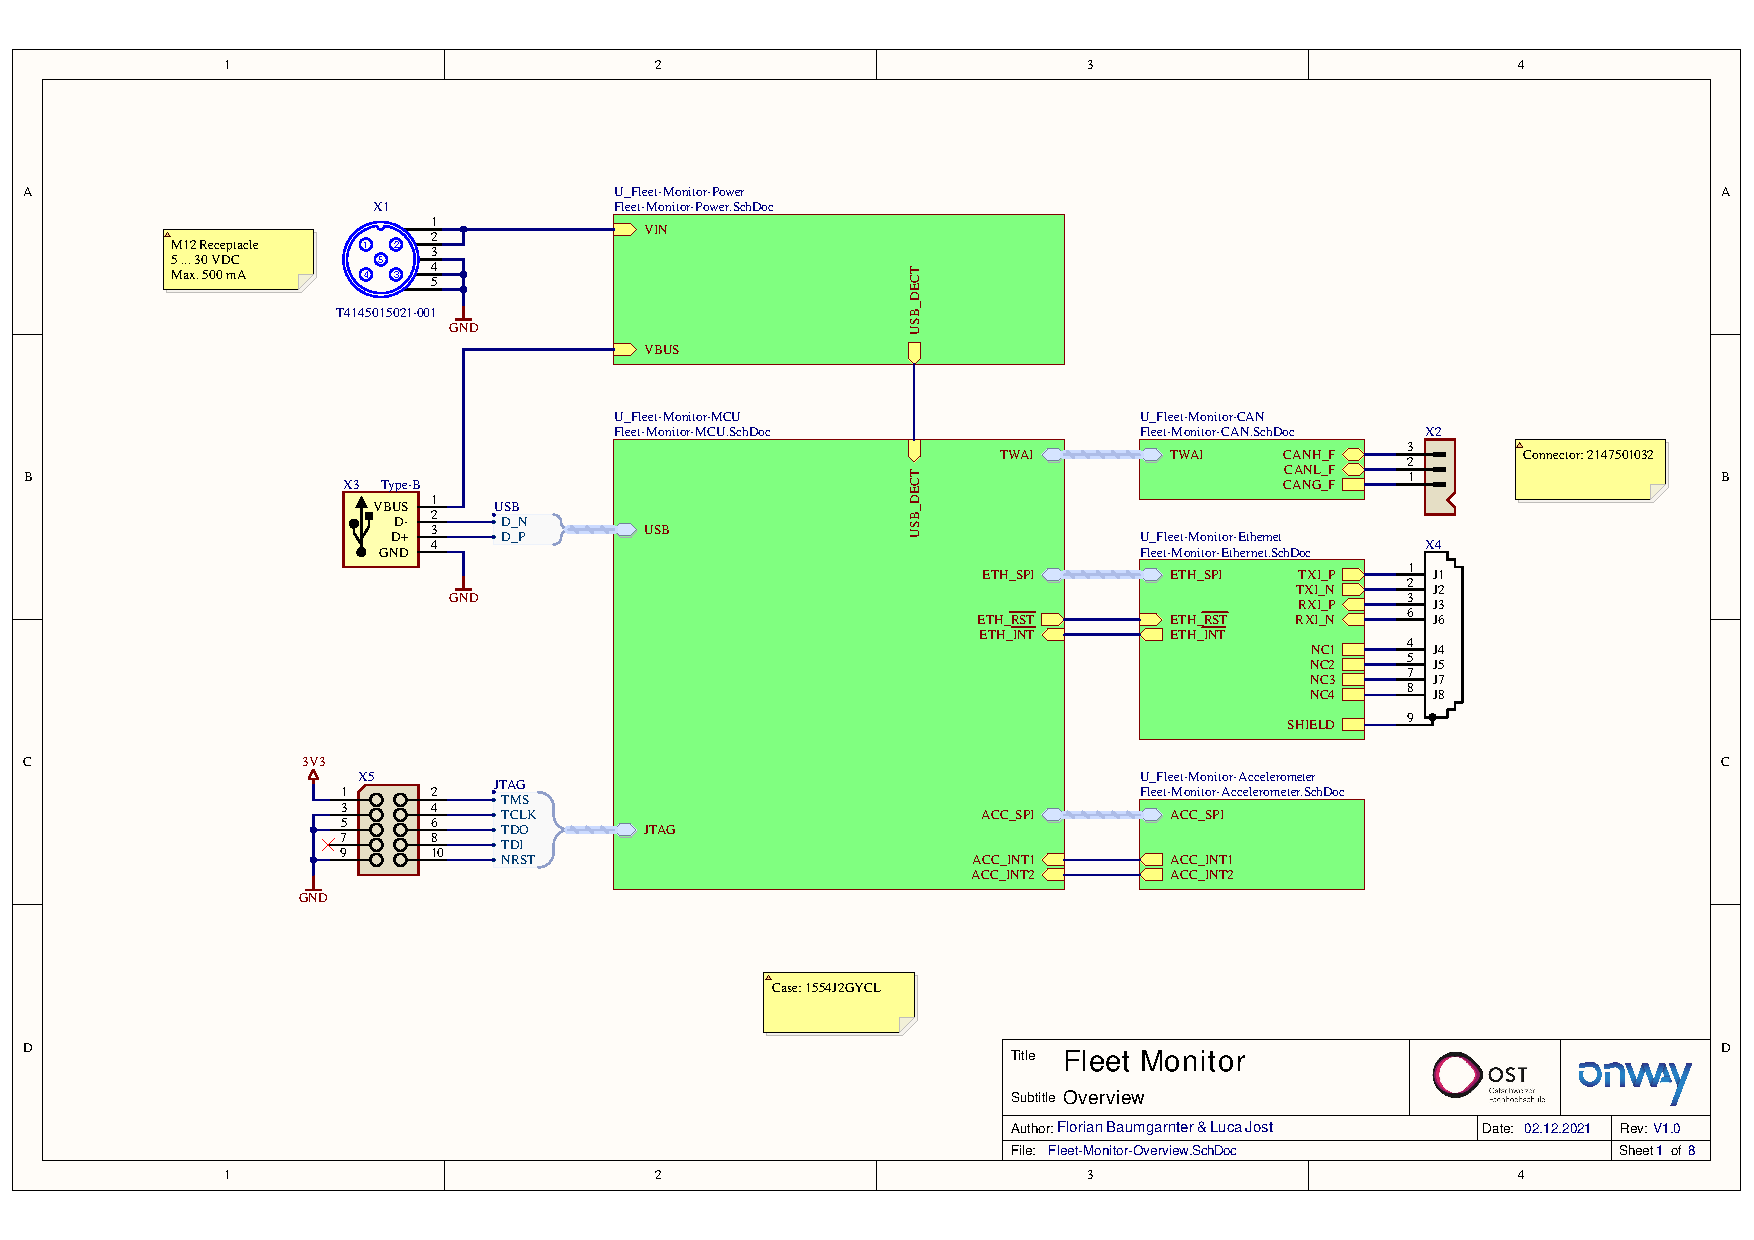
\includegraphics[angle=90, width=17.3cm, page=1]{appendix/Fleet-Monitor Schematics}}
\end{adjustwidth}
\newpage

\begin{adjustwidth}{0.23cm}{0cm} \hfuzz=7.0pt \vfuzz=20.0pt
\makebox[\textwidth]{\includegraphics[angle=90, width=17.3cm, page=2]{appendix/Fleet-Monitor Schematics}}
\end{adjustwidth}
\newpage

\begin{adjustwidth}{-0.23cm}{0cm} \hfuzz=7.0pt \vfuzz=20.0pt
\makebox[\textwidth]{\includegraphics[angle=90, width=17.3cm, page=3]{appendix/Fleet-Monitor Schematics}}
\end{adjustwidth}
\newpage

\begin{adjustwidth}{0.23cm}{0cm} \hfuzz=7.0pt \vfuzz=20.0pt
\makebox[\textwidth]{\includegraphics[angle=90, width=17.3cm, page=4]{appendix/Fleet-Monitor Schematics}}
\end{adjustwidth}
\newpage

\begin{adjustwidth}{-0.23cm}{0cm} \hfuzz=7.0pt \vfuzz=20.0pt
\makebox[\textwidth]{\includegraphics[angle=90, width=17.3cm, page=5]{appendix/Fleet-Monitor Schematics}}
\end{adjustwidth}
\newpage

\begin{adjustwidth}{0.23cm}{0cm} \hfuzz=7.0pt \vfuzz=20.0pt
\makebox[\textwidth]{\includegraphics[angle=90, width=17.3cm, page=6]{appendix/Fleet-Monitor Schematics}}
\end{adjustwidth}
\newpage

\begin{adjustwidth}{-0.23cm}{0cm} \hfuzz=7.0pt \vfuzz=20.0pt
\makebox[\textwidth]{\includegraphics[angle=90, width=17.3cm, page=7]{appendix/Fleet-Monitor Schematics}}
\end{adjustwidth}
\newpage

\begin{adjustwidth}{0.23cm}{0cm} \hfuzz=7.0pt \vfuzz=20.0pt
\makebox[\textwidth]{\includegraphics[angle=90, width=17.3cm, page=8]{appendix/Fleet-Monitor Schematics}}
\end{adjustwidth}
\newpage


\section{Fleet-Monitor V1.0 BOM} \label{Fleet-Monitor V1.0 BOM}
\enlargethispage{1.6cm}
\begin{adjustwidth}{-0.23cm}{0cm} \hfuzz=7.0pt \vfuzz=20.0pt
\makebox[\textwidth]{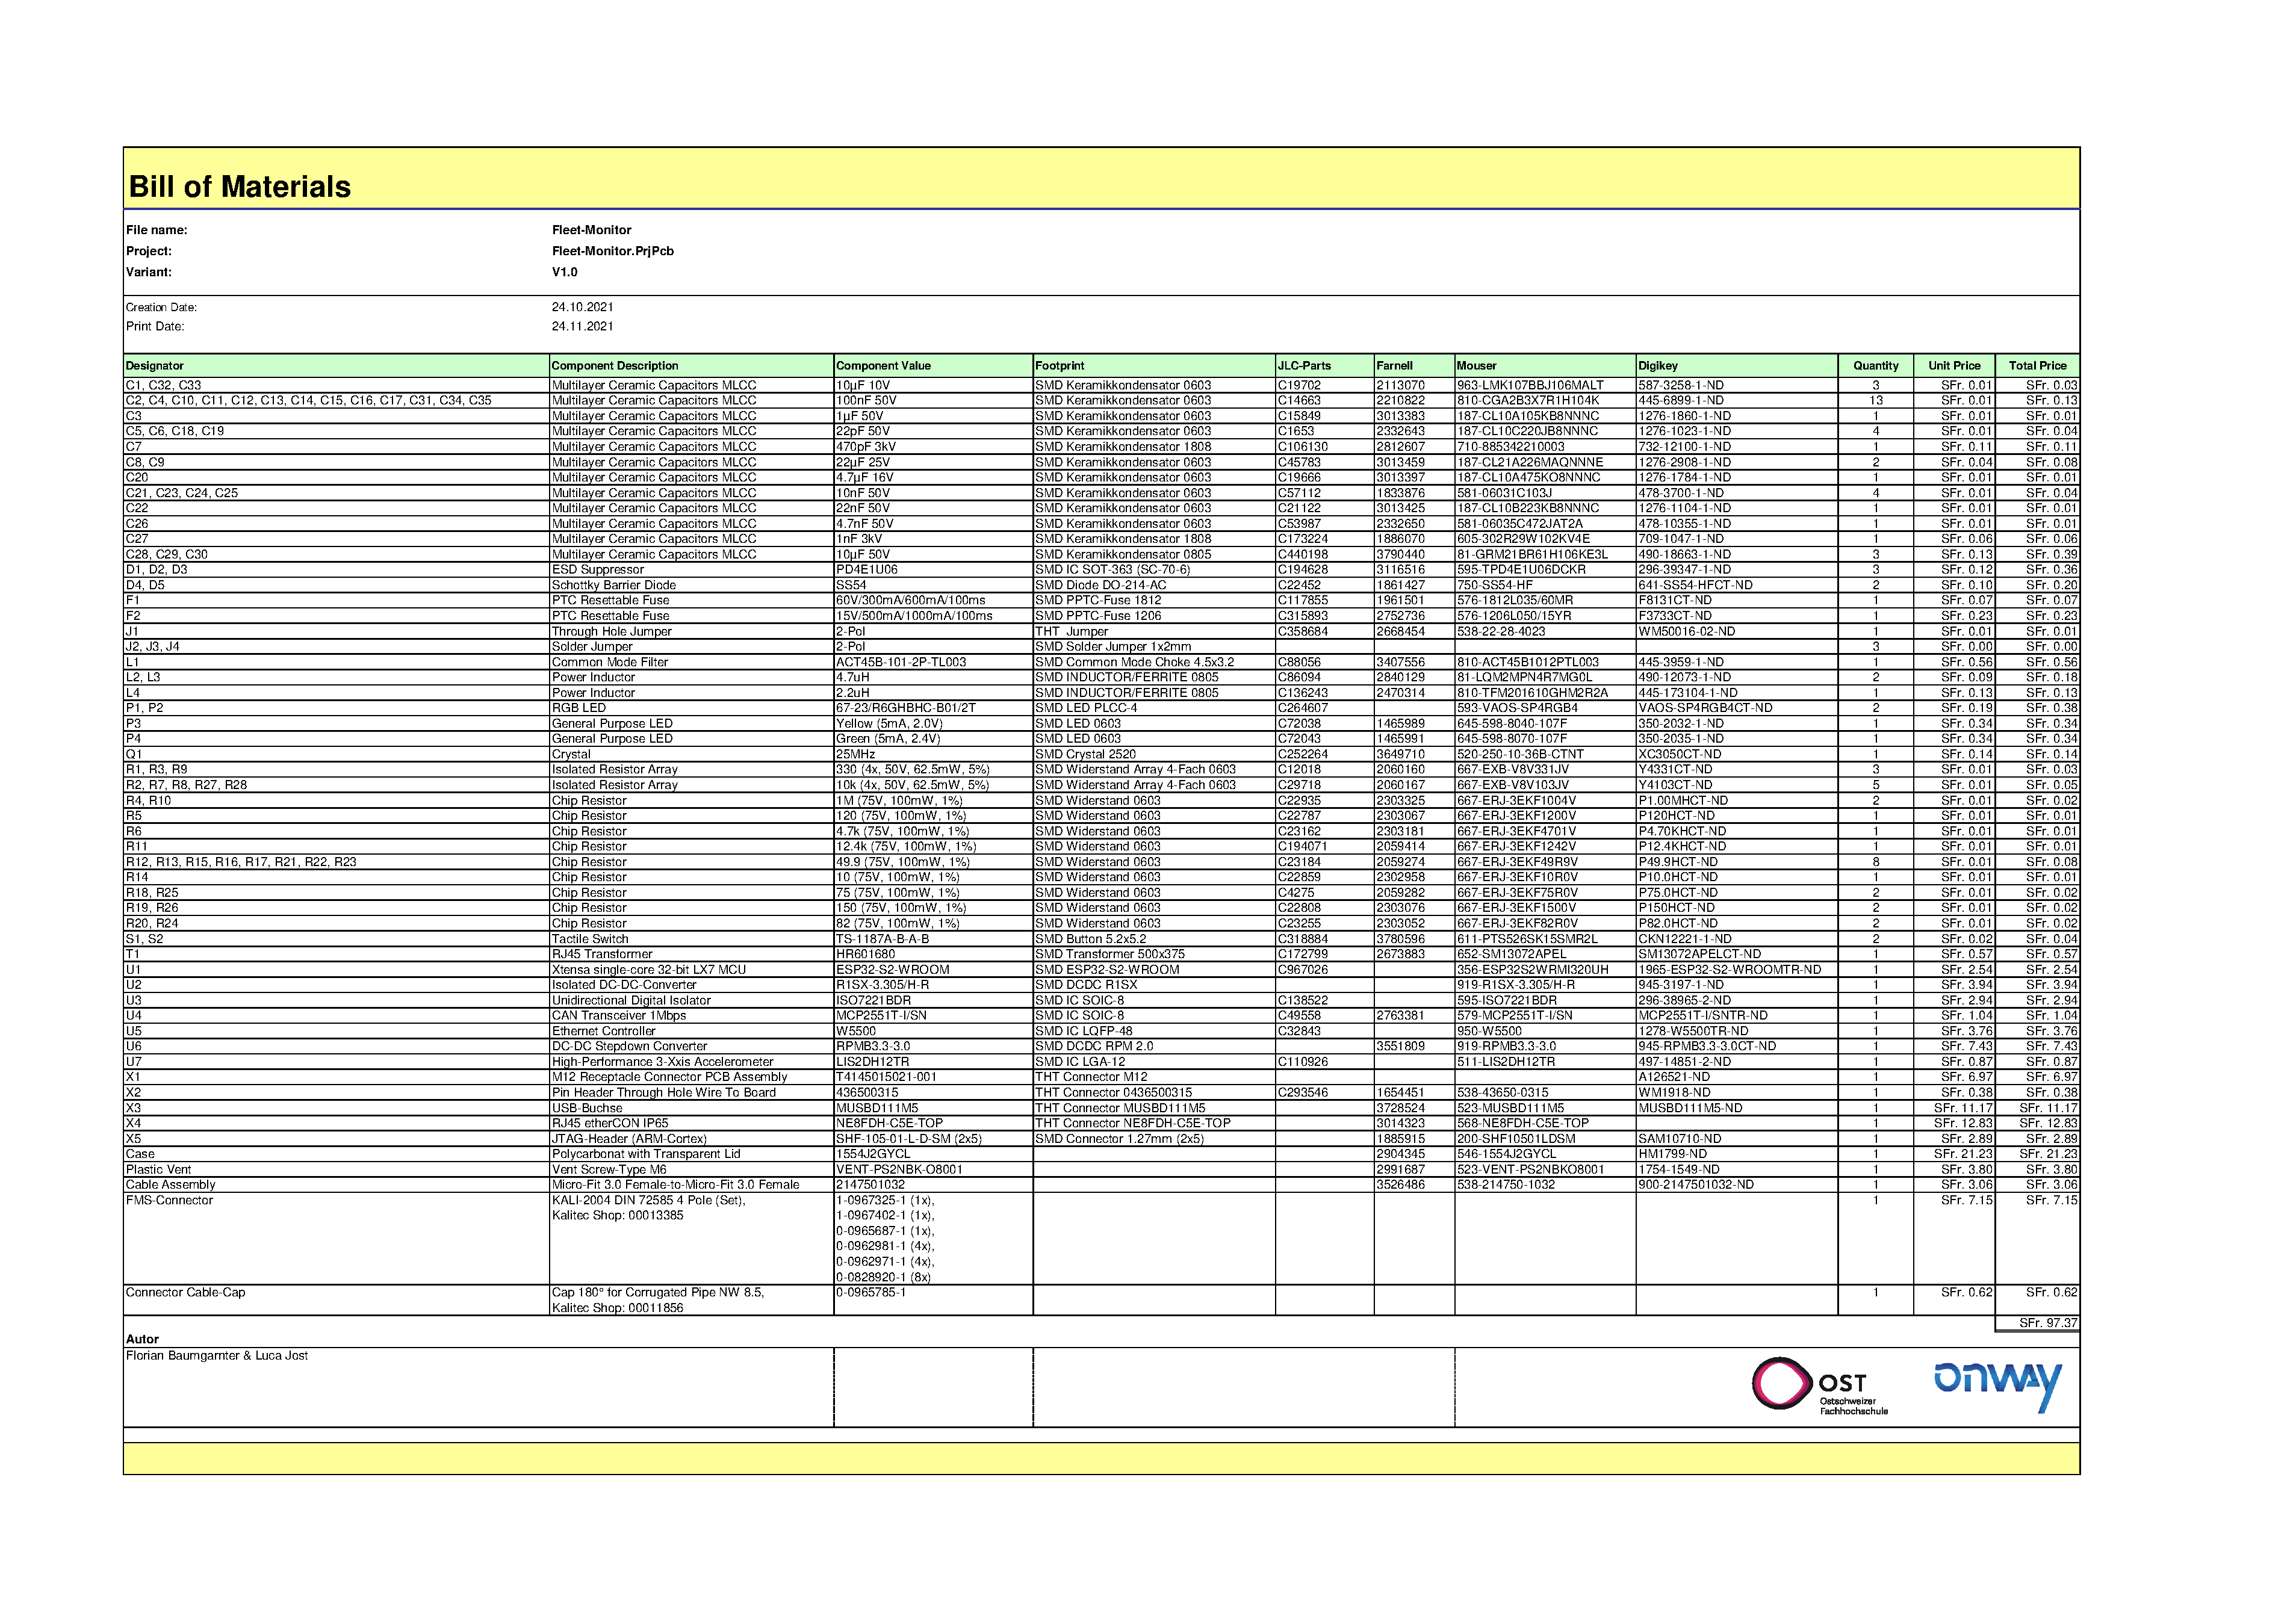
\includegraphics[angle=90, width=16.5cm]{appendix/Fleet-Monitor_BOM_croped}}
\end{adjustwidth}
\newpage


\section{Fleet-Monitor V1.0 PCB Layout} \label{Fleet-Monitor V1.0 PCB Layout}
\enlargethispage{2.5cm}
\begin{adjustwidth}{0.23cm}{0cm} \hfuzz=7.0pt \vfuzz=20.0pt
\makebox[\textwidth]{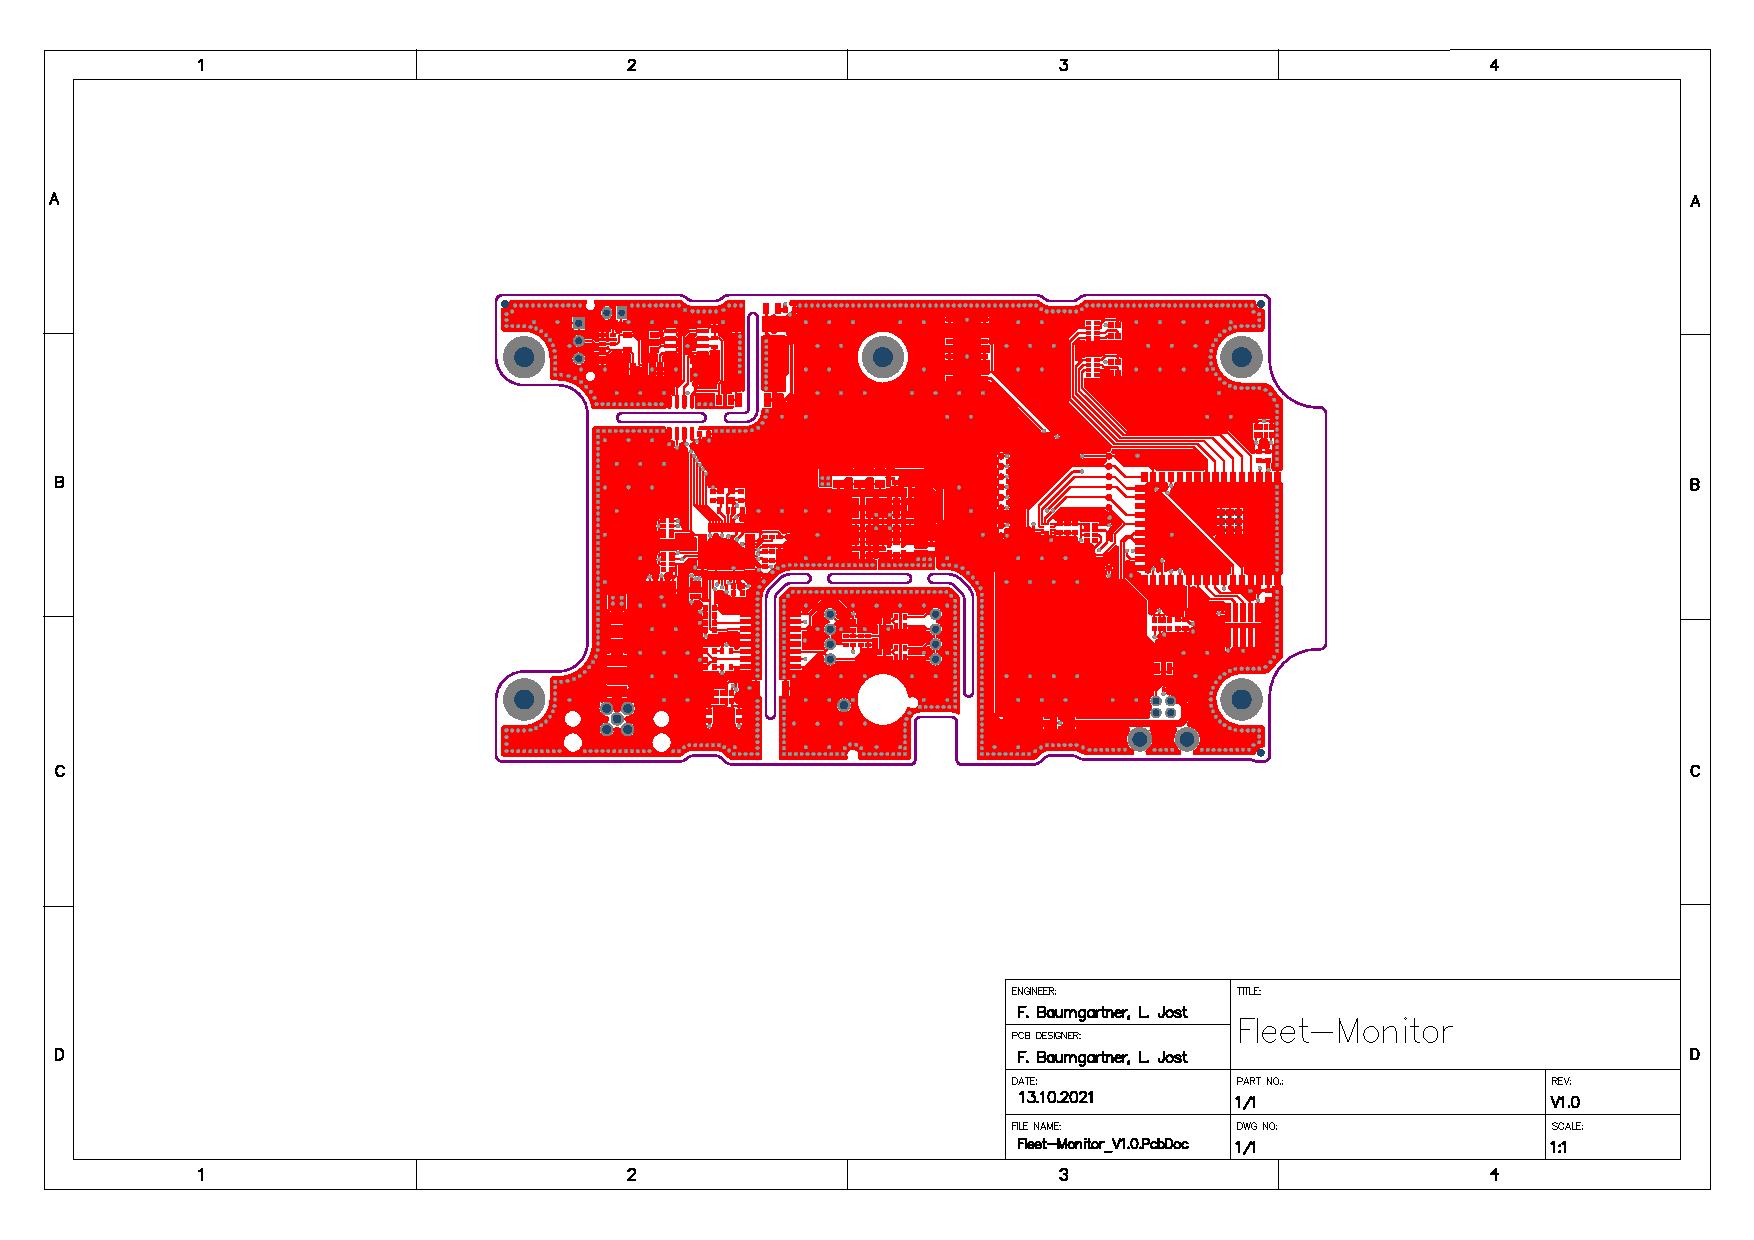
\includegraphics[angle=90, width=17.3cm, page=1]{appendix/Fleet-Monitor Layout}}
\end{adjustwidth}
\newpage

\begin{adjustwidth}{-0.23cm}{0cm} \hfuzz=7.0pt \vfuzz=20.0pt
\makebox[\textwidth]{\includegraphics[angle=90, width=17.3cm, page=2]{appendix/Fleet-Monitor Layout}}
\end{adjustwidth}
\newpage

\begin{adjustwidth}{0.23cm}{0cm} \hfuzz=7.0pt \vfuzz=20.0pt
\makebox[\textwidth]{\includegraphics[angle=90, width=17.3cm, page=3]{appendix/Fleet-Monitor Layout}}
\end{adjustwidth}
\newpage

\begin{adjustwidth}{-0.23cm}{0cm} \hfuzz=7.0pt \vfuzz=20.0pt
\makebox[\textwidth]{\includegraphics[angle=90, width=17.3cm, page=4]{appendix/Fleet-Monitor Layout}}
\end{adjustwidth}
\newpage

\begin{adjustwidth}{0.23cm}{0cm} \hfuzz=7.0pt \vfuzz=20.0pt
\makebox[\textwidth]{\includegraphics[angle=90, width=17.3cm, page=5]{appendix/Fleet-Monitor Layout}}
\end{adjustwidth}
\newpage

\begin{adjustwidth}{-0.23cm}{0cm} \hfuzz=7.0pt \vfuzz=20.0pt
\makebox[\textwidth]{\includegraphics[angle=90, width=17.3cm, page=6]{appendix/Fleet-Monitor Layout}}
\end{adjustwidth}
\newpage


\section{Fleet-Monitor V1.0 Mechanical Drawing} \label{Fleet-Monitor V1.0 Mechanical Drawing}
\enlargethispage{2.5cm}
\begin{adjustwidth}{0.23cm}{0cm} \hfuzz=7.0pt \vfuzz=20.0pt
\makebox[\textwidth]{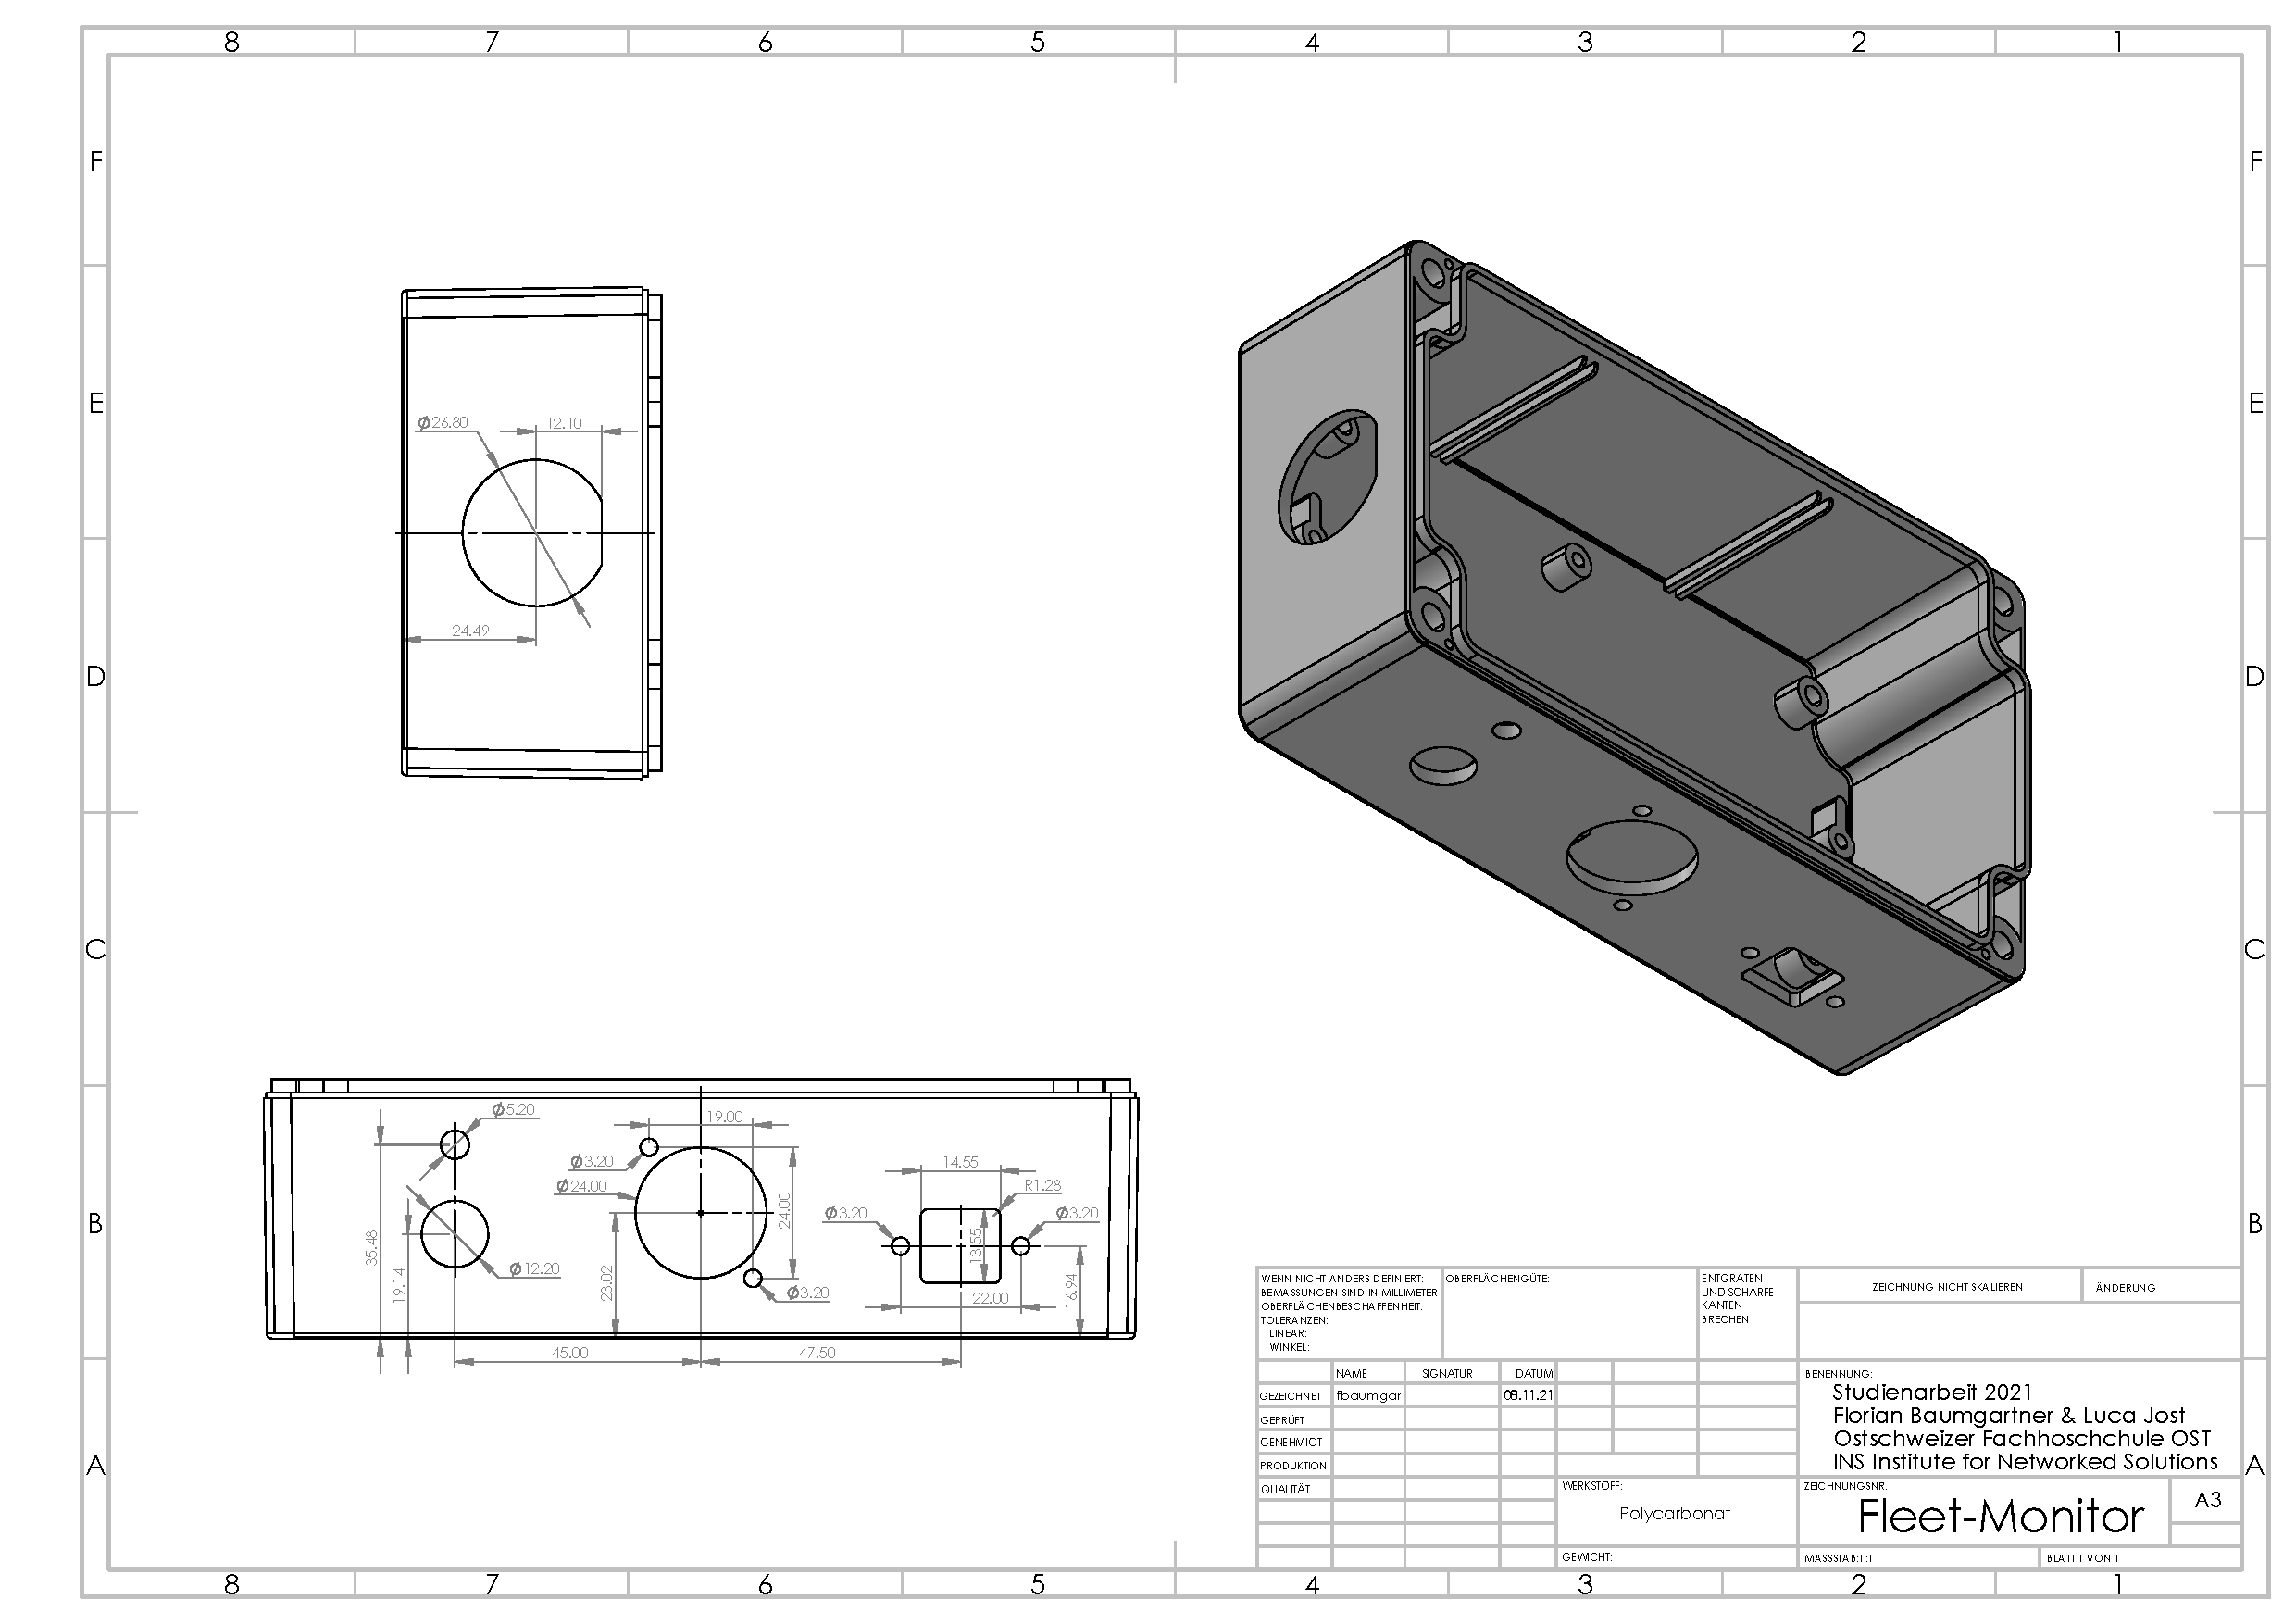
\includegraphics[angle=90, width=17.3cm, page=1]{appendix/Fleet-Monitor Case Drawing}}
\end{adjustwidth}
\newpage

\section{Test Reports} \label{Test Reports}

\subsection{Long Duration Test} \label{Long Duration Test}
\enlargethispage{2.5cm}
\begin{adjustwidth}{-0.23cm}{0cm} \hfuzz=7.0pt \vfuzz=19.0pt
\makebox[\textwidth]{\frame{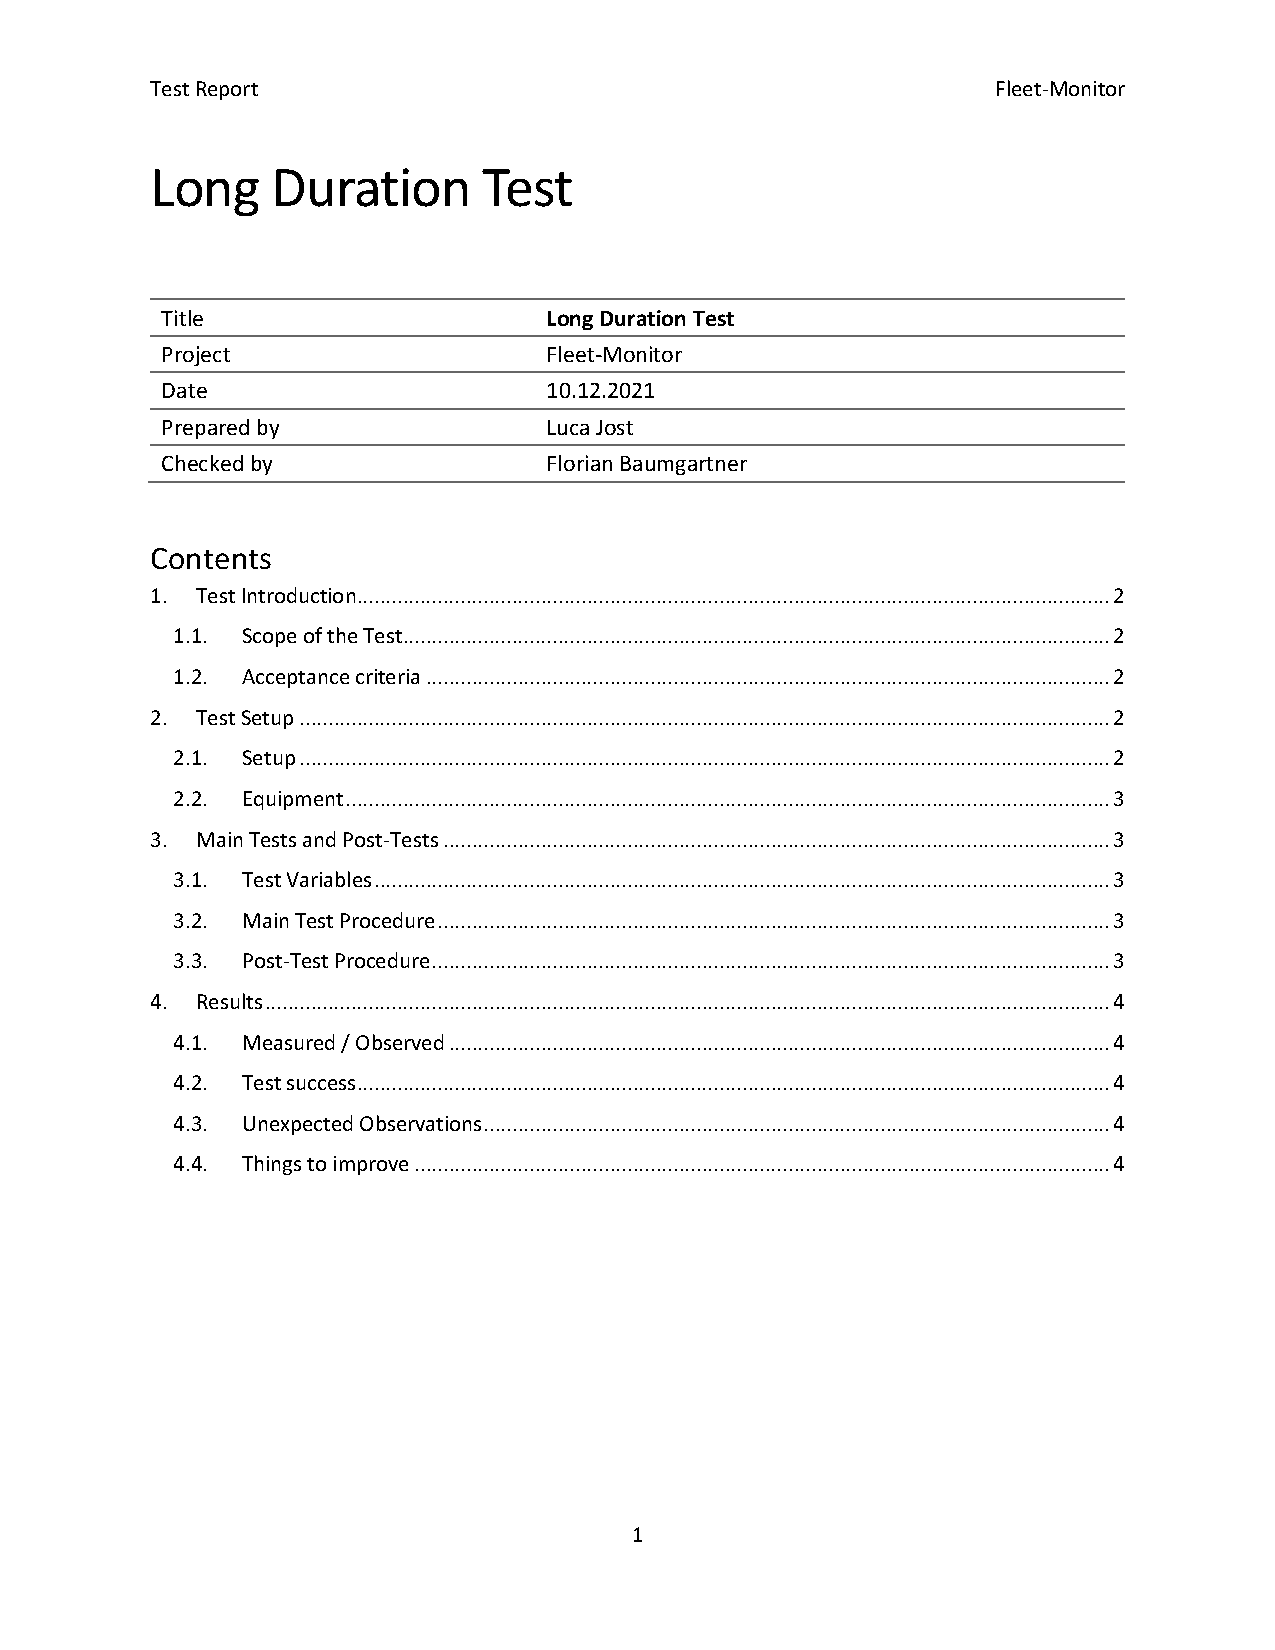
\includegraphics[width=17.3cm, page=1]{appendix/Long_Duration_Test}}}
\end{adjustwidth}
\newpage

\begin{adjustwidth}{0.23cm}{0cm} \hfuzz=7.0pt \vfuzz=19.0pt
\makebox[\textwidth]{\frame{\includegraphics[width=17.3cm, page=2]{appendix/Long_Duration_Test}}}
\end{adjustwidth}
\newpage

\begin{adjustwidth}{-0.23cm}{0cm} \hfuzz=7.0pt \vfuzz=19.0pt
\makebox[\textwidth]{\frame{\includegraphics[width=17.3cm, page=3]{appendix/Long_Duration_Test}}}
\end{adjustwidth}
\newpage

\begin{adjustwidth}{0.23cm}{0cm} \hfuzz=7.0pt \vfuzz=19.0pt
\makebox[\textwidth]{\frame{\includegraphics[width=17.3cm, page=4]{appendix/Long_Duration_Test}}}
\end{adjustwidth}
\newpage

\section{Financial Expenses} \label{Financial Expenses}
In table \ref{tab:financial-expenses} are the financial expenses listed of the project containing all development and production costs. Bills and other supporting documents can be found in the administrational repository (\ref{fleet-monitor-admin}) on GitHub. The total expenses of this project add up to a sum of \texttt{1’483.79} CHF.

\medskip
\begin{table}[h!]
    \hfuzz=23.0pt
    \begin{tabular}{ | p{8.2cm} | p{1.9cm} | >{\centering\arraybackslash}p{2.5cm} |} \hline
      \multicolumn{1}{|c|}{\textbf{Expense}} & \multicolumn{1}{c|}{\textbf{Date}} & \multicolumn{1}{c|}{\textbf{Value [CHF]}} \\ \hline 
      Adafruit & \centering 24.09.2021 & \texttt{271.50} \\ \hline
      DHL Fees & \centering 28.09.2021 & \texttt{ 39.40} \\ \hline
      Overleaf & \centering 30.09.2021 & \texttt{ 80.00} \\ \hline
      Kalitec Verbindungstechnik GmbH & \centering 12.10.2021 & \texttt{109.56} \\ \hline
      Aliexpress & \centering 13.10.2021 & \texttt{ 28.38} \\ \hline
      Post Zoll & \centering 20.10.2021 & \texttt{ 29.70} \\ \hline
      Thomann & \centering 21.10.2021 & \texttt{ 95.00} \\ \hline
      JLC-PCB & \centering 24.10.2021 & \texttt{213.80} \\ \hline
      JLC-PCB Extra Costs & \centering 25.10.2021 & \texttt{ 43.31} \\ \hline	
      Digikey & \centering 25.10.2021 & \texttt{400.35} \\ \hline
      Digitec & \centering 25.10.2021 & \texttt{ 82.55} \\ \hline
      DHL Fees & \centering 04.11.2021 & \texttt{ 38.10} \\ \hline
      LCSC & \centering 19.11.2021 & \texttt{ 52.14} \\ \hline
    \end{tabular}
    \caption{\label{tab:financial-expenses} Total Financial Expenses}
\end{table}
\newpage


\section{Data Archive} \label{Data Archive}
All created files and documents of this project are publicly available on GitHub. An institution called \textbf{SA-OST-2021} (\url{https://github.com/SA-OST-2021}) has been founded which contains repositories for each individual part of the project.
A quick description of the repositories including the associated web link is listed below:

\subsubsection{fleet-monitor-admin} \label{fleet-monitor-admin} \vspace{-0.2cm}
\begin{description}
  \item[Description:] This repository contains all confidential information of the project.\vspace{-0.25cm}
  \item[URL:] \url{https://github.com/SA-OST-2021/fleet-monitor-admin}\vspace{-0.25cm}
  \item[Type:] Private\vspace{-0.25cm}
\end{description}

\subsubsection{fleet-monitor-docs} \vspace{-0.2cm}
\begin{description}
  \item[Description:] This repository contains all additional documentation of the project.\vspace{-0.25cm}
  \item[URL:] \url{https://github.com/SA-OST-2021/fleet-monitor-docs}\vspace{-0.25cm}
  \item[Type:] Public\vspace{-0.25cm}
\end{description}

\subsubsection{fleet-monitor-requirements-specification} \vspace{-0.2cm}
\begin{description}
  \hfuzz=35.0pt
  \item[Description:] This repository contains the Requirements Specification.\vspace{-0.25cm}
  \item[URL:] \url{https://github.com/SA-OST-2021/fleet-monitor-requirements-specification}\vspace{-0.25cm}
  \item[Type:] Public\vspace{-0.25cm}
\end{description}

\subsubsection{fleet-monitor-report} \vspace{-0.2cm}
\begin{description}
  \hfuzz=35.0pt
  \item[Description:] This repository contains this document.\vspace{-0.25cm}
  \item[URL:] \url{https://github.com/SA-OST-2021/fleet-monitor-report}\vspace{-0.25cm}
  \item[Type:] Public\vspace{-0.25cm}
\end{description}

\subsubsection{fleet-monitor-hardware} \vspace{-0.2cm}
\begin{description}
  \item[Description:] This repository contains hardware and mechanical related documents.\vspace{-0.25cm}
  \item[URL:] \url{https://github.com/SA-OST-2021/fleet-monitor-hardware}\vspace{-0.25cm}
  \item[Type:] Public\vspace{-0.25cm}
\end{description}

\subsubsection{fleet-monitor-embedded} \vspace{-0.2cm}
\begin{description}
  \item[Description:] This repository contains firmware source code written in C++.\vspace{-0.25cm}
  \item[URL:] \url{https://github.com/SA-OST-2021/fleet-monitor-embedded}\vspace{-0.25cm}
  \item[Type:] Public\vspace{-0.25cm}
\end{description}

\subsubsection{fleet-monitor-configuration-tool} \vspace{-0.2cm}
\begin{description}
  \item[Description:] This repository contains the filter configuration tool written in Python.\vspace{-0.25cm}
  \item[URL:] \url{https://github.com/SA-OST-2021/fleet-monitor-configuration-tool}\vspace{-0.25cm}
  \item[Type:] Public\vspace{-0.25cm}
\end{description}

\subsubsection{fleet-monitor-network-tool} \vspace{-0.2cm}
\begin{description}
  \item[Description:] This repository contains the network tool (server) written in Python.\vspace{-0.25cm}
  \item[URL:] \url{https://github.com/SA-OST-2021/fleet-monitor-network-tool}\vspace{-0.25cm}
  \item[Type:] Public\vspace{-0.25cm}
\end{description}

\subsubsection{fleet-monitor-visualizer} \vspace{-0.2cm}
\begin{description}
  \item[Description:] This repository contains the graphical data visualizer written in Python.\vspace{-0.25cm}
  \item[URL:] \url{https://github.com/SA-OST-2021/fleet-monitor-visualizer}\vspace{-0.25cm}
  \item[Type:] Public\vspace{-0.25cm}
\end{description}

\subsubsection{fleet-monitor-rasp-image} \vspace{-0.2cm}
\begin{description}
  \item[Description:] This repository contains an image of the Raspberry Pi SD-Card.\vspace{-0.25cm}
  \item[URL:] \url{https://github.com/SA-OST-2021/fleet-monitor-rasp-image}\vspace{-0.25cm}
  \item[Type:] Public\vspace{-0.25cm}
\end{description}
